\documentclass[a4paper]{article}

% Typesetting
%\usepackage{mathpazo}
\usepackage{geometry}
\usepackage{hyperref}
\usepackage{setspace}
\usepackage[activate={true,nocompatibility},final,tracking=true,kerning=true,spacing=true,factor=1100,stretch=20,shrink=20]{microtype}
\microtypecontext{spacing=nonfrench}
\hyphenpenalty=5000
\tolerance=1000
\usepackage{listings}
\usepackage{pdfpages}
\usepackage{tabularx} % in the preamble
\usepackage{setspace}
\addtocontents{toc}{\protect\enlargethispage{\baselineskip}}

% Graphics
\usepackage{graphicx}
\graphicspath{{./images/}}

% Tables
\usepackage{booktabs}

% Utility
\usepackage{url}
\usepackage{amssymb}
\usepackage{amsmath}
\usepackage{amsfonts}
\usepackage{subfigure}
\usepackage{algorithm}
\usepackage{algorithmic}
\usepackage{enumerate}
\usepackage{eulervm}
\usepackage{tikz}
\usepackage{xcolor}
\usepackage{color}
\usepackage{todonotes}

\renewcommand{\algorithmiccomment}[1]{\hfill// \textit{#1}}

\usepackage{framed, color}
\definecolor{shadecolor}{rgb}{0.8, 0.9, 1.0}

% Science Units
\usepackage{textcomp}
\usepackage[]{siunitx}
\sisetup{tophrase=--}
\sisetup{repeatunits=false}
\usepackage{latexsym}

% Bibliography (Use \citep)
\usepackage[]{natbib} %numbers
\setlength{\bibsep}{3.5pt}

\begin{document}

% Title Page
\newgeometry{margin=3cm}
\thispagestyle{empty}
\begin{center}
% StarFish Logo
\includegraphics[width=\linewidth]{logo_starfish_project}\\\vspace{1cm}

% Subtitle
{\large
Finding implicitly related items based on semantic similarities and metadata in a non-hierarchical network of documents
}\\\vspace{0.5cm}

% Authors
\begin{tabular*}{0.8\linewidth}{@{\extracolsep{\fill}}lcr}
& \textbf{Authors} & \\
\hline
R. van Ginkel 	& J. Peters 	& L. Weerts \\
\end{tabular*}
\\\vspace{2cm}
% Company
Project commissioned by \emph{Perceptum B.V.}\\\vspace{1cm}

% Supervisors
\textbf{Supervisors}\\
\begin{tabular}{r|l}
Academic Supervisor & Raquel Fernandez \\
Company Supervisors & Robrecht Jurriaans \\
& Sander Latour \\
& Wijnand Baretta
\end{tabular}


% UvA
\vfill
\today\\
Universiteit van Amsterdam

\end{center}
\restoregeometry

\clearpage

% Front Matter
\begin{abstract}
This report describes the results of the second year's project for the Perceptum team. The project focused on creating a \emph{document link recommender system} to the document knowledge base of the Starfish website, a platform where educators can share information about educational innovation. Because users of Starfish do not have knowledge of all the documents in the entire knowledge base, a system that can perform this automatically is needed. This report describes the implementation and analysis of several algorithms that can perform this task. 

To create the document linker, a document descriptor-based technique was used. Firstly, each of the documents is transformed into a descriptor by algorithms called \emph{vectorizers}. Six vectorizers were implemented. Two vectorizers are based on the text of documents (textvectorizer and weighted text vectorizers) and two others use the tags of documents (simple tag similarity and tag smoothing). The last two vectorizers perform the textual transformation on text-based descriptions of tags (glossaries of tags and weighted tags). Additionally, a hybrid method of a text-based and tag-based is proposed. After creating the document descriptors, a ranking is made of all documents based on the similarity of the document descriptors and the descriptor of the new added document. This was done using the $K$-Nearest Neighbor algorithm with several distance metrics, of which the cosine distance turned out to work the best. The system also provides a method that can re-rank this set of proposed documents based on the probability that two documents are linked together.  The last step in the pipeline determines how many of the nearest neighbours should be returned. For this a threshold was set that compares the distance as calculated with $K$-Nearest Neighbor of two documents with consecutive ranks. 

Three main conclusions were drawn from this study. Firstly, the
text vectorizers performs the best if the newly added document is a Question (42.02-44.82\% accuracy on k-link measuring). However, it cannot deal with
documents that have different languages or non-textual documents such as images, videos
and audio. The simple tag vectorizer has the
best performance (22.80\% overall average accuracy on k-link measuring) and is the fastest. The best overall performance with the k-link measurement
is gained with the hybrid vectorizer (26.13\%) that uses the textvectorizer if no tags are
available and the simple tag vectorizer otherwise. This vectorizer performs as
good on most document types as the simple tag vectorizer, but performs significantly
better on questions (31.93\% versus 16.67\%). Secondly the probabilistic model of the network that is proposed 
is either to simplistic
or the data available is too little. In either case it might be off interest to
further investigate a similar model on a bigger data set. Lastly the method
of selecting the number of documents shows that the overall performance 
does not change significantly if the threshold is added to most vectorizers.
However, the text vectorizers seem to have a bias towards a higher precision in the
trade off between precision and recall. The
glossaries of tags and weighted glossaries of tags get a higher
recall for persons. The best performance while using the threshold was obtained
using the hybrid vectorizer, with an average precision, recall and F1 measure of respectively 28.61\%, 27.26\% and 23.92\%. 

These results are clearly not good enough for an automatic linking system, but could be considered high enough for a recommender system since they are far above guessing level. It is now up to the client to choose if a precision of 28.61\% is good enough to let the user select a document to link and if a recall of 27.26\%
covers enough of the documents within the knowledge base.  
\end{abstract}
\clearpage

\tableofcontents
\clearpage

% Main Matter
% The introduction (dah)

% DO NOT COMPILE THIS FILE DIRECTLY!
% This is included by the other .tex files.

\section{Introduction}

This report describes the results of the Second Year's project of the Perceptum team. The project focused on creating a \emph{document link recommender system} to the StarFish website. 

StarFish, one of the projects of Perceptum, is a website that aims to share knowledge about the education domain by means of a connected graph. People from all around the world should get access to this knowledge graph in a simple, personalized manner. The nodes in this graph are documents and they are connected with links. These documents can be of all sorts of types - e.g. a good pratice, information, a question. Each document has a set of tags assoicated with it, which describe the different aspects of educational innovation. StarFish is community-driven: both the content of the documents as the links between documents are determined by the users of StarFish. 

The drawback of a community driven knowledge graph is that not all the users know the entire document base. Especially when the knowledge base grows it becomes impossible for a user, since one does not know the existence of one or more linkable documents. A possible solution could be to make use of administrators, which can devote more time in getting to know all the documents, but that approach has two main drawbacks. First of all, this would mean that some central authority determines whether or not two documents should be linked. This is not in line with the idea of a community-driven knowledge base. Secondly, if the knowledge base grows even further, it becomes impossible also for an administrator to keep track of all documents. Imagine one person having to link all pages on Wikipedia - an impossible job. 

In order to overcome the problem of linking documents in a large knowledge base, this process should be automated. This project therefore focuses on automating making the connections between documents. Though ideally these connections should be made completely automatic, a first step would be to create a recommendation system. When a user adds a new document, he or she can choose from a list of proposed documents the documents he or she deems relevant. This means that the recommendor system does not have to work perfect, but should work reasonably well enough. Defining 'well enough', however, is also a part of this project. Thus, the product vision of the system can be described in the following concise way:

\begin{shaded}
\textbf{{\large Product vision:}} \vspace{0.5\baselineskip} \hrule
	\begin{description}
 		\item[For] StarFish users
 		\item[who] search for and edit knowledge in starfish
 		\item[the] starfish document linker 
 		\item[is] a starfish core system addition
 		\item[that] finds related documents
 		\item[unlike] moderated or individual linking
 		\item[our] product uses algorithms and data to suggest document links 
	\end{description}
\end{shaded}


Within the time span of this project multiple ways of recommending links between documents have been explored. The results of these explorations will be discussed in this report. 

\section{Product overview}

The product created in this project is a python program takes a set of documents and a new document and returns the subset of documents that should be linked with the new document. For this, a descriptor-based approach was used, which consists of three steps. First, each of the documents is transformed into a descriptor: a vector containing numerical values that in some way describes the document (hence the term 'descriptor'). Creating these discriptors is not trivial and during the project several techniques have been explored. Secondly, a ranking is made of all documents based on the similarity of the document descriptors and the descriptor of the new added document. To compare the descriptors the Nearest Neighbour algorithm was implemented, including five different distance metrics that determine how near two vectors are. Thirdly, an algorithm chooses the proper amount of proposed links that must be returned.

\begin{lstlisting}
python documentlinker.py -vectorizer <vectorizername> 
-distance <distance metric> -threshold <'auto' or a fixed number>
\end{lstlisting}

We will now discuss each of these parameters, since these will give more insight into the approach that was chosen to solve the problem. For the performance of the different parameters we refer to the evaluation section. 

\subsection{Vectorizer}
The first step is to create document descriptors, which is done by algorithms that we call \emph{vectorizers}. Two main paths have been explored: transformation based on text and transformation based on tags.

\subsubsection{Text-based transformation}
\begin{description}
\item [Textvectorizer] The text-based vectorizers use the textual content of the documents and are therefore generally applicable to other systems. The textual content is first transformed into a \emph{bag of words}. Then, based on all the documents in the knowledge base, the \emph{TF-IDF} value is calculated for each of the words in the bag of words. \emph{TF-IDF} stands for Term Frequency-Inverse Document Frequency and is a number that represents the importance of a word to a document in a bigger set of documents. Thus, the document descriptor consists of a vector with all TF-IDF values for that document of all words in the corpus. 

\item[Weighted\_textvectorizer] The weighted textvectorizer is implemented as an extention of the textvectorizer. Besides the descriptor of a document itself, this method also adds the vectors of documents linked to it with some weight. This captures the idea that if a new document resembles some of the documents that are linked to one particular document, it is more likely to be linked to this particular document. 
\end{description}

\subsubsection{Tag-based transformations}
\begin{description}
\item[Simple\_tag\_similarity] The tag-based transformations are more StarFish specific, since they make use of the tags that are assigned to the documens. A tag is a keyword that describes a topic/term that is important for that document. For example, 'Online Support and Online Assessment for Teaching and Learning Chemistry' is tagged with 'chemistry', 'e-learning' and 'assessment'. The simple tag similarity vectorizer creates a vector where each value indicates whether or not one particular tag is assigned to the document. 

\item [Tag\_smoothing] The tag smoothing vectorizer uses the co-occurence of tags in estimating document similarity. % PLEASE EXPLAIN

\item [Glossaries\_of\_tags] Another way of capturing tag similarity is by using tag Glossaries. Most of the tags have a Glossary - a special type of Document which holds an explanation of a tag. Though glossaries are documents, they cannot be assigned as a link since this should be done by assigning a tag. The glossaries can still be used by applying a text-based transformation on the glossaries to indicate the similarity between tags. Thus, glossaries\_of\_tags can be seen as a hybrid form of the tag and text-based approaches, where the glossary of a tag is turned into a TF-IDF bag of words. The document descriptor consists of the sum of vectors of each of it's tags. 

\item [Weighted\_tag\_vectorizer] This is an extension of glossaries of tags, where a weight is assigned to the tag vectors. % PLEASE EXPLAIN
\end{description}

\subsubsection{StarFish specific adaptations}
\begin{description}
\item[Bayesian Weigthed Vectorizer] Both the tag-based and text-based approaches uses some kind of 'semantic similarity' - the similarity of tags or text. However, except for the weighted text vectorizers, no information about possible links is used. For example, the text on a person's profile might be similar to other persons, but within StarFish a person is almost never linked to another person. In the Bayesian Weigthed Vectorizer this is captured by weighting the vectors with the probability that two documents are linked together:
\begin{align}
\nonumber P(D_a \rightarrow D_b | t)
\end{align}
Thus, the weight of a tag within a vector is equal to the chance that given this particular vector, a document of type a (the type of the newly added document) and a document of type b (equal to the type of proposed link) are linked together.
\end{description}

\subsection{Distance}
The nearest neighbour algorithm loops through all available document descriptors and compares these with the descriptor of the new document. The closer related the descriptors are, the higher their ranking will be. The distance metrics define the closeness of the descriptors - a lower distance means a closer relation. The following were implemented:

\begin{description}
\item[Eucledian]
\item[Cosine]
\item[Bhattacharyya]
\item[Correlation]
\item[Intersection]
\end{description}

\subsection{Threshold value}
In the end, an algorithm chooses the proper amount of proposed links that must be returned. If the threshold value is set to a fixed number, e.g. 10, than only the  proposed links of rank 1-10 are returned. If the threshold is set to \emph{'auto'}, the number of returned links is based on the gradient of the distances. For example, if the algorithm is only certain that the first two links are correct, it returns no more than two links. For user-friendliness a maximum of 15 links is returned. 

% Domain (what are we dealing with and why is it non-trivial

% DO NOT COMPILE THIS FILE DIRECTLY!
% This is included by the other .tex files.

\section{Domain}
The Starfish website aims to be a platform for educators where educational innovations and projects can be shared. Because many teachers have different vocabulary and diverse questions, a strict hierarchical structure of the shared content is a problem. Starfish tries to overcome this by structuring it's knowledge base in a non-hierarchical manner. There are sub communities within Starfish which gives learners the opportunity to share knowledge that is specific to their faculty or institution. 

The knowledge base itself consists of one big set of entities. These entities are called documents. Currently, the Starfish knowledge graph contains 240 documents. These documents can be of a variety of types. Each document in this graph is of one of the following types: Information, Glossary, Question, Good Practice, Project, Person or Event. Documents have an author, title, text, tags and links. The Person type is an exception on that and has a name-field instead of title and a about-field instead of text. Some document types have different optional fields like `headline' for good practices and projects. The graph is structured by directional links between documents.  On average a document 3.9 links.

Each document in the knowledge base is assigned a set of tags based on the different aspects of educational innovation the document covers. On average a document has 3,4 tags. Glossaries are special types of documents, as they are description for tags. This means that it is unnecessary for the link recommendation system to return glossaries, since a glossary could are `linked' via the assigned tag. Because different groups use alternative names to describe concepts, tags can be aliases of each other. For this project, aliased tags are regarded as one single tag. Of the 210 tags the current system contains, 146 unique tag concepts can be distinguished of which 24,6\% have a glossary. 

These numbers and properties of the system give some insight into the current
state of the dataset and possible solutions. The major part of Starfish data is
text-based, so semantical document analysis could be performed with standard
text processing techniques. The tags of documents could also give insight into
the semantics of the documents. Additionally, the links that are currently in
Starfish can be used as guidelines on when documents should be linked and when
not. 

Although Starfish aims to be user-driven, user voting will not be explored in this 
project. This was not part of the initial request and Starfish is currently to small 
for such an endeavor. The data for this is not at hand and there are too little
users to test effectively. 


% Theory (how could this problem theoretically be solved)
\section{Theory}

In solving the linking problem, one must find a way to compare different documents based on their linkability with a newly added documents. Computationally, this can be done by creating document descriptors - vectors that the describe the features of a document in some way. This opens the path for three major research directions. The first two are a text-based and tag-based approach towards creating document descriptors. Thirdly, the known distribution of links between document types within the current Starfish knowledge base can be used to determine the prior probability of proposed documents. These three directions will be discussed in the following sections. 

\subsection{Graphs}

\subsection{Text-based descriptors: bag of words and TF-IDF}
One way of capturing the semantic similarity of two text document is by comparing the TF-IDF values of their contents. If two documents cover the same subject(s), they are likely to contain similar keywords. To capture this similarity, the documents can be transformed into a list of all words that are present within that text. This is called a bag-of-words representation. Instead of counting the frequency of each word within a document, the more sophisticated Term Frequency-Inversed Document Frequency value can be used. TF-IDF is a statistic that reflects the importance of a word in a document within a corpus and can be calculated as follows:

\begin{align}
\nonumber {tf}(t,d) = 0.5 + \frac{0.5 \times {f}(t, d)}{\max\{{f}(w, d):w \in d\}}\\
\nonumber {idf}(t, D) =  \log \frac{N}{|\{d \in D: t \in d\}|}\\
\nonumber {tfidf}(t,d,D) = {tf}(t,d) \times {idf}(t, D)
\end{align}

The TF-IDF induces a trade off between the term frequency, the number of times a word appears in a document, and the inverse document frequency, the inverse of how often a word is used in the entire corpus. Words such as 'and', 'or', and 'of' will have a high term frequency within a document. However, their inversed document frequency will be very low, since they occur very often within the entire corpus. Infrequent used words such as Starfish are less likely to occur within a corpus, so if they do occur often within one particular document the TF-IDF value will be high. 

\subsection{Nearest Neighbor and distance metrics}
The 



\subsection{Document descriptors and Nearest Neighbor}
Once the document descriptors have been created


% What have we actually implemented
\section{Product overview}

The product created in this project is a python program takes a set of
documents and a new document and returns the subset of documents that should be
linked with the new document. For this, a descriptor-based approach was used,
which consists of three steps. First, each of the documents is transformed
into a descriptor. Second, a ranking is made of all documents based on the
similarity of the document descriptors and the descriptor of the new added
document. This was done using the $K$-Nearest Neighbor algorithm with several
distance metrics. Lastly, an algorithm chooses the proper amount of proposed
links that must be returned. We will now discuss each of these steps, since these will give more
insight into the approach that was chosen to solve the problem. For the
performance of the different algorithms we refer to the experiment section. 

\subsection{Vectorizer}
The first step is to create document descriptors, which is done by algorithms that called \emph{vectorizers}. Two main paths have been explored: transformation based on text and transformation based on tags.

\subsubsection{Text-based transformation}
\begin{description}
\item [Textvectorizer] The text-based vectorizers use the textual content of the documents and are therefore generally applicable to knowledge bases that contain text-based documents. The textual content is first transformed into a bag of words. Then, based on all the documents in the knowledge base, the \emph{TF-IDF} value is calculated for each of the words in the bag of words.  

\item[Weighted\_textvectorizer] The weighted textvectorizer is implemented as an extension of the textvectorizer. First, all descriptors of the documents are calculated similarly as in the textvectorizer. Then each document descriptor is recursively increased with the sum of the descriptors of it's links, decreased by some weight parameter. This captures the idea that if a new document resembles some of the documents that are linked to one particular document, it is more likely to be linked to this particular document. 
\end{description}

\subsubsection{Tag-based transformations}
\begin{description}
\item[Simple\_tag\_similarity] The tag-based transformations are more Starfish specific, since these make use of the tags that are assigned to the documents - Starfish feature. A tag is a keyword that describes a topic/term that is important for that document. For example, `Online Support and Online Assessment for Teaching and Learning Chemistry' is tagged with `chemistry', `e-learning' and `assessment'. The simple tag similarity vectorizer creates a vector where each value indicates whether or not one particular tag is assigned to the document. 

\item [Tag\_smoothing] The tag smoothing vectorizer uses the co-occurence of tags in estimating document similarity. Even though tags might not co-occur on any document in the data set, they can still provide information about each other. For example, the dataset consists of documents with associated tags like $\{\{t_1, t_2\}, \{t_1, t_3\}\}$. From the co-occurence it does not follow that $t_2$ and $t_3$ are related, however by transitivity with $t_1$ we want to create a small implicit link between $t_2$ and $t_3$. The tag smoothing method does this based on work from \citet{zhou2011web}.

\item [Glossaries\_of\_tags] Another way of capturing tag similarity is by using tag Glossaries. They can be used by applying a text-based transformation on the glossaries to find similarities between tags. Thus, glossaries\_of\_tags can be seen as a hybrid form of the tag and text-based approaches, where the glossary of a tag is turned into a TF-IDF bag of words. The document descriptor consists of the sum of vectors of each of its tags. 

\item [Weighted\_tag\_vectorizer] This is an extension of glossaries of tags.
  In the original glossaries of tags, it is assumed all tags contribute the
  same amount of information to a document's links. In practice some tags
  provide more information than others. If a certain tag is on nearly all
  documents in the dataset, it does not provide a lot of insight into linking
  new documents. In contrast a tag which is only attached to a small subset of
  documents is much more informative. The weighted tag vectorizer creates
  descriptors by summing the tag vectors with a weight based on the frequency
  of that tag in the dataset. The intuition for this is the same as that
  of the TF-IDF bag of words approach for creating vector representations
  of a text.

\item [Hybrid] The hybrid vectorizer is a combination of the text and simple tag vectorizers. If a document does not have tags, the textvectorizer is used. Otherwise, the simple tag vectorizer is used to propose document links.
\end{description}

\subsection{Distance}
A ranking is created using the $K$-Nearest Neighbor algorithm that sorts the
document descriptors based on their distances with the newly added document.
The following five distance metrics were implemented. These are discussed
in section~\ref{sec:metrics}

\begin{itemize}
\item Eucledian
\item Cosine
\item Bhattacharyya
\item Correlation
\item Intersection
\end{itemize}

The cosine distance is the default value, since that one seems to perform the
best on the Starfish knowledge graph based on our experiments. 
More on this in section~\ref{sec:experiments}. 

\subsection{Starfish specific adaptations: Bayesian weighting}
Both the tag-based and text-based approaches use some kind of `semantic similarity' - the similarity of tags or text. However, except for the weighted text vectorizers, no information about possible links is used. For example, the text on a person's profile might be similar to other persons, but within Starfish a Person document is almost never linked to another Person. To make more use of known links within the Starfish knowledge base, the ranking of document descriptors as created by $K$-Nearest Neighbor can be re-ranked using the probability that two documents are linked together given their tags:
\begin{align}
\nonumber P(D_a \rightarrow D_b | t)
\end{align}
Thus, the weight of a tag within a vector is equal to the chance that given this particular vector, a document of type a (the type of the newly added document) and a document of type b (equal to the type of proposed link) are linked. The inverse of an approximation of this probability is multiplied with the distances that come from $K$-Nearest Neighbor in order to enlarge the distance of proposed links that are unlikely given the Starfish knowledge base. 

\subsection{Threshold value}
The next step in the pipeline is to determine how many of the nearest neighbours should be returned. Depending on the application of the Starfish document linker, the desired number might vary. If one wants to immediately link the results, the certainty for relatedness should be high. If the links are presented to a user which can approve or reject them, the relatedness may be lower. Currently, this is configurable by setting a threshold parameter between 0 and 1. Zero will only return the closest document, 1 will return almost all. After exploration of the dataset the default value is 0.3, which roughly returns the same amount of links which is currently average in Starfish.

\subsection{Output}
The document linker can be run using the documentlinker.py file. There are two ways in which the results of the document linker are reported: a JSON file with the proposed links and a textual performance report. The JSON file can be viewed using \emph{view.html}, a HTML page that can be opened in a browser. A file can be selected using the `choose file'-button. The HTML page then displays a list of all documents. The content and proposed links can be viewed by clicking on the corresponding buttons. The grey links indicate False Negatives, the green ones True Positives and the red ones False Positives. 

The performance reports is displayed in the terminal and shows the precision and accuracy (see the metric section in experiments) of the entire knowledge base and per document type. It also gives insight into the distribution of document types by presenting the percentages one type linked to another. For example, a percentage of 85\% on the Person row and Question column indicates that of all Person documents, 85\% of the links from a Person to another document types directed to Questions. 


% Very specific explanation of each of the algorithms in the pipeline and their pro's and cons
\section{Method}

\subsection{Data preprocessing}
Starfish text content is serialized as HTML, a format which is not suitable for
calculating semantical similarity. Before processing, the data is sanitized by
removing HTML tags and entities and convert unicode characters to their closest
ASCII representation.


Maybe something about creating the folds by removing some of the documents?

\subsection{Text descriptors}
\subsubsection{Textvectorizer}

The first set of vectorizers focuses on the texts of the documents. The
\emph{textvectorizer} is a very generic approach that can be used on any corpus
of textual documents. In the Starfish context, we define 'content' as the title
and text-fields of a document. The only exception on this are Persons, of which
we wil use the name and about-fields. 

The textvectorizer first transforms the set of documents into a bag of words
and calculates the TF-IDF values for all words. This was done using the
TFIDFVectorizer of scikitlearn \citep{scikit-learn}.  Though the TF-IDF values
of words that are used very often should be low, common words such as 'and',
'or' and 'of' are still present in the vectors. This could be caused by the
different types of documents. For example, a Question often structured in a
less complex way than a Project description. To prevent this from happening,
the English stopword list that comes standard with scikit learn was used to
remove these words from the document descriptors.

\subsubsection{Weighted textvectorizer}
The weighted text vectorizer is an extension of the textvectorizer that takes
into account the links of the proposed documents. The vectors of the links of a
document are added with some weight to the vectors of the documents themselves.
Intuitively, this would add semantic information about a document based on it's
links. For example, a Person is likely to write other documents about his or
her subjects of expertise. Knowing not only the biography of a Person, but also
the content he or she has added to Starfish, gives a more complete image of
what documents could be related to that Person.

The vectors of links of a document are added in a recursive way, where
documents that are linked directly have a higher weight than documents that are
linked transitively. The algorithm is displayed in figure xx.

\subsection{Tag descriptors}
\subsubsection{Simple tag vectorizer}
The tag-based approach is more Starfish specific than the text-based approach,
since it depends on the tags that are available in Starfish. The tags on
Starfish are added by the users themselves, so offer a human-based vision on
what a document is really about. The simple tag vectorizer is a very straight
forward implementation of the idea of using tags. The vectors of this
transformation consist of a binary list that tells whether or not a tag is
attached to the document. 

\subsubsection{Tag smoothing}
The tag smoothing vectorizers creates descriptors based on the tag set of a
document. A tag co-occurs with other tags in a document, we assume documents
with similar tags should be linked in Starfish. Let the frequency of occurrence
with other tags across the dataset will form a vector for each tag. The
descriptor for a document is then created by combining the occurrence vectors
for all the document's tags. Now documents with tags that occur together will
be seen as similar.

There are two reasons why one would like to smooth the tag co-occurences.
Firstly, a problem for this is that tags must occur together before the
algorithms works properly. The Starfish dataset contains a lot of tags that
only occur with a small frequency, which means the tag occurrence vector will
contain many zeros. This makes the algorithm perform bad with little data.
Secondly, two tags can describe the same concept and be connected to that
concept through a common co-occurence with another tag. Whilst they describe
the same concept and are connected to that, they are not directly linked
together. Therefore it seems feasible to perform some sort of smoothing on the
co-occurences of tags.

\citet{zhou2011web} proposed a method to cluster web documents based on tag set
similarity. This is based on a similarity between two tags as a relation
between the frequency these tags occur separate and together, as described in
equation~\ref{eq:tag_similarity}. To smooth these similarities between tags, a
tag similarity matrix $\mathcal{C}$ is constructed. Each entry $c_{i,j}$ in
this matrix can be viewed as the angle $\theta_{i,j}$ between two unknown
vectors $v_i$ and $v_j$. These vectors cover both explicit similarity and
implicit similarity \citep{park2010vector}. This transfers the problem to find
a set of linearly independent vectors $\{v_1,v_2,\ldots,v_n\}$ for which for
all $v_i \cdot v_j = \cos(\theta_{i,j})$. One must find a matrix $\mathcal{V}$
for which $V^TV = C$. This can be done by orthogonal triangularization on
$\mathcal{C}$ for which \citeauthor{zhou2011web} introduces a modified Cholesky
transform.

\begin{equation} \label{eq:tag_similarity}
s_{i,j} = \frac{f_{i,j}}{f_i + f_j - f_{i,j}}
\end{equation}


\subsubsection{Glossaries of tags}
The glossaries of tags approach is also based on the intuition that certain
tags cover overlapping concepts. Just like the simple tag vectorizer the
glossaries of tags approach exploits this intuition. In the Starfish system a
tag is expected to have a glossary; a short English description of the concept
of a tag. These glossaries contain terms and words that are descriptive for the
tag. The glossary of tags vectorizer aims to use these terms to create a
document descriptor based on the tags associated with a document. In other
words the set of

First for each tag a tag descriptor $t_i$ is created. This tag descriptor is
a TF-IDF bag of words vector created from the glossaries of each tag. These
descriptors form the basis for the document descriptors. For each document
a document descriptor $d_i$ is created by summing the tag descriptors of the
associated tags.
\begin{align}
  d_i = \sum_{j \in T(d_i)} t_j
\end{align}
where $T(d_i)$ is the set of tag indices associated with document $d_i$. This
way a document descriptor is created based on a semantic representation of
the tags associated with the document.

\subsubsection{Weighted tag vectorizer}
The weighted tag vectorizer is similar to the glossaries of tags vectorizer
discussed in the previous section. However instead of just summing the tag
descriptors an weight is used to scale the tag descriptor. This way tags that
are associated with a lot of documents don't contribute as much to the document
descriptor as tags that are only associated with a few documents. The weight
$w_t$ for each tag descriptor $t$ is based on the number of documents that the
tag is associated with. $w_t$ is defined as follows
\begin{align}
  w_{t_i} = 1 - \frac{\textrm{Number of documents associated with $t_i$}}{\textrm{Total number of documents}}
\end{align}
With this weight the weighted tag document descriptor $d_i$ can be computed
in the following way:
\begin{align}
  d_i = \sum_{j \in T(d_i)} w_{t_j}t_j
\end{align}
This vectorizer first gives extra importance to descriptive words in each of
the tag descriptors by using the TF-IDF bag of words. After this more
importance is given to tags that are more descriptive using the weights. This
results in a document descriptor that has high weights for words that are
descriptive for tags that are descriptive for the document.

\subsection{Bayesian weighting}
Up to this point only the semantic similarity of documents has been taken into
account. This does however, not take the information in the current network
into account. For example the probability of a document of type information
linking to a document of type information is higher than that of the same
document linking to a document of type project. For this $P(d_i \to d_j \mid
\Sigma_{ij})$ and $P(d_i \to d_j)$ are interessting. Or in other words the
probability that two documents are linked given the number of tags they have in
common and the probability that two document of a given type are linked. These
probabilies can be estimated from the data. First it is shown how to compute
$P(d_i \to d_j \mid \Sigma_{ij})$.

\begin{align}
  P(d_i \to d_j \mid \Sigma_{ij}) &= \frac{P(\Sigma_{ij} \mid d_i \to d_j)P(d_i \to d_j)}{P(\Sigma_{ij})} \\
  P(\Sigma) &= \frac{{D_\Sigma \choose 2}}{{|D| \choose 2}} \\ 
  P(\Sigma \mid d_i \to d_j) &= \frac{\textrm{Number of links that have $\Sigma$ tags in common}}{|L|} \\
  P(d_i \to d_j) &= \frac{|L|}{{|D| \choose 2}}
\end{align}
Where $L$ is the set of all links and $D$ is the set of all documents.
$\Sigma_{ij}$ is the number of tags that document $d_i$ and $d_j$ have in
common. As is shown above $P(d_i \to d_j)$ is computed as a uniform probability
for all documents. However this can also be computer while taking the document
types into account. This is computed next:
\begin{align}
  P(d_i \to d_j) &= \frac{|L|}{{|D| \choose 2}}
\end{align}
These probabilities will be used to scale the distances that are
computed by the nearest neighbor algorithm. Because the distances for documents
that have a high probability should be low therefore the final distances are
computed in the following way:
\begin{align}
  d_i = (1 - P(d_i\to d_j \mid \Sigma_{ij})) \times (1-P(d_i \to d_j)) \times \delta_i
\end{align}
where $\delta_i$ is the distance as computed by the nearest neighbor algorithm
and $d_i$ the final distance that is used to select the proposed documents to
be linked. This may seem a rather simple statistical model, however due to the
limited set of items in the dataset it is very hard to learn a more complicated
model.

\subsection{Thresholds}
After creating the descriptors for a document and finding a new document's
nearest neighbors, a subpart of those links needs to be returned by the linker
application. An average document in Starfish has x links. To create a dynamic
threshold which returns similar a similar amount of documents, a document from
the Starfish data is extracted and then to re-inserted to test the number of
links the system returns to the number of links the document had in the
original system. Figure~\ref{fig:link_histogram} shows the distribution of
outgoing links in the current network.

\begin{figure}[h]
\centering
\includegraphics[width =0.45\textwidth]{images/link_histogram}
\caption{The frequency of outgoing links in Starfish documents}
\label{fig:link_histogram}
\end{figure}

The the threshold should depend on multiple factors which mostly depend on the setting in which the document linker will be used. Two major factors determine how the threshold should work.
\begin{enumerate}[1.]
	\item The degree of certainty we expect from the returned documents.
	\item The maximum number of documents that should be returned for a specific application.
\end{enumerate}
If the system is used to directly create the links into the Starfish system, the first aspect is very important. Only documents with a very high degree of linking certainty should then be returned, the amount should be based on the contents of the current system. If the system will be used to create recommendations which a user must accept or reject, the first aspect becomes less important and the system should return an amount of links which can quickly be reviewed by users. To ensure the flexibility for choice of algorithm and integration of the application, the threshold algorithm will contain a configurable parameter.

When adding a document to Starfish, it is assumed that there is always at least one related document. Based on the distance of the nearest neighbor for the new document, the index of a and the configurable parameter, the threshold is defined as in equation~\ref{eq:thresh}. In this equation, $\alpha$ is the configurable parameter, $m$ is the number of documents returned by the nearest neighbor algorithm, $d_0$ is the distance to the closest document, $\frac{m - n}{m}$ is a factor that ensures the maximum allowed distance decreases for documents ranked further away. This is based on the differences between two nearest neighbors which are visualized in figure~\ref{fig:thresholds_differences}. The distances have a long tail form: the distances between the nearest neighbors is relatively large for the closest documents and smaller between the documents further away. 

\begin{equation}
t_n = \alpha (1 - d_0) \frac{m - n}{m}
\label{eq:thresh}
\end{equation}


% Overview of experiments done on the entire pipeline
\section{Experiments}
\subsection{Evaluation metrics}
In order to evalute the performance of the different algorithms, three different metrics were used. For each of these methods we hold on to the closed world assumption that if a link is not present within the given data set, it should not be a link. 

\subsubsection{Precision and recall}
Precision and recall can be calculated when the complete system pipeline is used. Precision reflects the fraction of relevant documents from all proposed documents and can thus be calculated as follows:

\begin{align*}
  \textrm{precision} = \frac{|\;\textrm{relevant\;documents} \cap \textrm{retrieved\;documents}\;|}{|\textrm{retrieved\;documents}\;|}
\end{align*}

Recall represents the fraction of relevant documents of all originally linked documents and can be calculated as follows:

\begin{align}
  \nonumber \textrm{recall} = \frac{|\;\textrm{relevant\;documents} \cap \textrm{retrieved\;documents}\;|}{|\;\textrm{relevant\;documents}\;|}
\end{align}
The precision and recall can be unraveled into precision and recall per document type to give more insight into the performance of the algorithms with regards to different document types. 

\subsubsection{K-links}
The k-links metric is used to evaluate the algorithms, without being influenced by the threshold for the number of proposed links. For a document with a given number of correct links, it proposes the same amount of links that the document is known to have. This evaluation metric thus makes the assumption that the algorithm knows in advance how many links should be returned. By doing so, the recall and precision are equivalent since the number of relevant and retrieved document is the same. It prevents the precision of being too optimistic, which would be the case if the fixed number would be lower than the actual amount of links. It also prevents the recall for being too optimistic in the cases that the actual amount of links is lower than the fixed number of proposed links. 

The disadvantage of the k-links metric is of course that it does not take into account the certainty the algorithm has due to the distances. For example, it could be that the distance of the first two ranked documents is very small, but the distance of the third is very large. If the original document has 10 links, the system is forced to additionally return the nine documents, even though these are likely to be wrong because they have a relatively big distance. 

\begin{table}

\begin{tabular}{| l | l | l | l | l | l | l | l |}
\hline
{\bf CORRELATION} & Inf. &  Question &  Good Pr.& Project & Person &  Event & {\bf Average} \\
\hline
Textvectorizer & 20.93 & 34.12 & 30.36 & 24.85 & 7.09 & 21.43 & {\bf 18.82} \\ 
Weighted text & 20.36 & 39.56 & 30.36 & 16.04 & 7.09 & 21.43 & {\bf 19.02} \\ 
Simple tag & 53.02 & 16.67 & 46.53 & 49.96 & 26.15 & 33.73 & {\bf 35.31} \\ 
Tag smoothing & 51.23 & 21.93 & 21.43 & 41.04 & 23.59 & 42.06 & {\bf 33.82} \\ 
Glossaries of tags & 15.03 & 15.35 & 32.14 & 25.73 & 7.95 & 35.71 & {\bf 14.52} \\ 
Weighted tag & 0 & 0 & 0 & 0 & 0 & 0 & {\bf 0} \\ 
\hline
\\
\hline
{\bf COSINE} & Inf. &  Question &  Good Pr.& Project & Person &  Event & {\bf Average} \\
\hline
Textvectorizer & 20.49 & 40.70 & 30.36 & 25.42 & 5.81 & 21.43 & {\bf 19.49} \\ 
Weighted text & 21.67 & 44.82 & 30.36 & 16.04 & 5.81 & 21.43 & {\bf 19.90} \\ 
Simple tag & 21.21 & 16.67 & 69.64 & 37.81 & 17.53 & 46.83 & {\bf 22.80 } \\ 
Tag smoothing & 20.58 & 21.93 & 44.64 & 31.04 & 13.59 & 46.83 & {\bf 20.69} \\ 
Glossaries of tags & 18.68 & 16.67 & 48.21 & 31.46 & 10.51 & 40.48 & {\bf 18.02} \\ 
Weighted tag & 0 & 0 & 0 & 0 & 0 & 0 & {\bf 0} \\ 
\hline
\\
\hline
{\bf INTERSECTION} & Inf. &  Question &  Good Pr.& Project & Person &  Event & {\bf Average} \\
\hline
Textvectorizer & 4.16 & 3.51 & 10.71 & 19.06 & 0 & 24.21 & {\bf 4.45} \\ 
Weighted text & 4.15 & 3.51 & 10.71 & 19.1 & 0.00 & 24.21 & {\bf 4.45} \\ 
Simple tag & 4.15 & 3.51 & 10.71 & 19.1 & 0.00 & 24.21 & {\bf 4.45} \\ 
Tag smoothing & 4.15 & 3.51 & 10.71 & 19.1 & 0.00 & 24.21 & {\bf 4.45} \\ 
Glossaries of tags & 4.16 & 3.51 & 10.71 & 19.06 & 0.00 & 24.21 & {\bf 4.45} \\ 
Weighted tag & 4.15 & 3.51 & 10.71 & 19.1 & 0.00 & 24.21 & {\bf 4.45} \\ 
\hline
\\
\hline
{\bf EUCLIDEAN} & Inf. &  Question &  Good Pr.& Project & Person &  Event & {\bf Average} \\
\hline
Textvectorizer & 3.04 & 3.95 & 17.86 & 0 & 0.85 & 21.43 & {\bf 3.25} \\ 
Tag smoothing & 1.32 & 1.32 & 7.14 & 0 & 0.43 & 0 & {\bf 1.08} \\ 
Simple tag & 14.05 & 10.53  & 30.36 & 38.23 & 14.36 & 35.71 & {\bf 16.56} \\ 
Tag smoothing & 0 & 0 & 0 & 0 & 0 & 0 & {\bf 0} \\ 
Glossaries of tags & 15.64 & 10.53 & 41.07 & 31.46 & 7.95 & 40.47 & {\bf 14.75} \\ 
Weighted tag & 0 & 0 & 0 & 0 & 0 & 0 & {\bf 0} \\ 
\hline
\\
\hline
{\bf BHATTACHARYYA} & Inf. &  Question &  Good Pr.& Project & Person &  Event & {\bf Average} \\
\hline
Textvectorizer & 15.57 & 35.88 & 30.36 & 16.15 & 5.30 & 21.43 & {\bf 16.19} \\ 
Weighted text & 18.72 & 29.04 & 30.35 & 11.99 & 7.95 & 21.43 & {\bf 16.63} \\ 
Simple tag & - & - & - & - & - & - & {\bf -} \\ 
Tag smoothing & 4.16 & 3.51 & 10.71 & 19.06 & 0 & 24.2 & {\bf 4.44} \\ 
Glossaries of tags & 18.36 & 17.98 & 48.21 & 48.13 & 10.51 & 40.45 & {\bf 19.39} \\ 
Weighted tag & 0 & 0 & 0 & 0 & 0 & 0 & {\bf 0} \\ 
\hline
\end{tabular}

\caption{Performance k-link measuring of all vectorizers with each of the distance metrics per document type}
\label{klink}
\end{table}

\subsection{Text-based descriptors}
Table \ref{klink} shows the k-link values of all vectorizers, including those of the textvectorizer and the weighted-text vectorizer. The best performance of the textvectorizers is obtained by the cosine distance. This can be attributed
 to the fact that the cosine distance is independent to document length and only
 computes a simmilarity in document structure. In other words when a document
 has the exact same words as a seconds document but only twice as much the
 cosine similarity classifies these documents as exactly equal. As the textvectorizer
 encodes the number of word occurences in a vector the cosine distance can 
 easily find document that use the same words frequently.

The cosine distance metric gives the best results for the text vectorisers. On average, 19.49\% and 19.59\% percent of the number of proposed links respectively are correct. The weighted text vectorizer performs a bit better, which is mainly due to an improvement in performance on information and questions. % ROBBERT, FIND SOME QUALTITATIVE EXAMPLES FOR THIS. 

Both textvectorizers have a low percentage correct with regards to proposing links for Persons. A further analysis shows that 76.36\% (not weighted) and 69.09\% (weighted) of the links for Persons are towards other Persons (see appendix X). However, within the Starfish network such links almost never occur (see table \ref{bayes_table3} for the distribution of document types within Starfish). This could explain the low performance on persons. 

Overall, both textvectorizers are slow in performance even though the corpus is small. Additionally, the the bag-of-words approach imposes a few limitations on the document linker. Firstly, it performs bad when different languages are used. Figure x shows the differences of vectors of three texts when an English document is combined with an English proposed document and a Dutch proposed document. In the case of two different languages, there are less words that the two documents have in common. If important keywords entail word such as 'clickers' versus 'stemsysteem', there is no way of relating the two documents. Secondly, the current StarFish network consists of mainly textual content. However, in the future this is likely to be extended with images, videos and other non-textual content. These sources should then somehow be converted to text.

\subsection{Tag-based descriptors}

\subsubsection{Simple tag similarity vectorizer}
The performance of the simple tag similarity vectorizer, as shown in table \ref{klink} together with the other tag vectorizers, is about 26\% precision when measuring k-link. The unraveling per document type shows that Question documents and Person documents perform the least. This can be explained by the fact that half of both Questions and Persons have zero tags. Obviously, the simple tag vectorizer cannot deal with such documents. In fact, almost all other Questions have only one tag. Since the simple tag vectorizer compares vectors, it wil prefer documents that also have only that particular tag, which makes it sensitive to attaching Questions to Questions. Something similar seems to happen with Persons, of which 50.91\% of the connections are with other Persons. Apparently, persons with similar expertise are tagged similarly. However, as mentioned with the text vectorizer, in Starfish persons almost never refer to other persons. Moreover, if a document is badly labeled this can also induce problems. For example, take the question 'Is there an English version in Tentamenlade', tagged with 'ToetsenEnToetsgestuurdleren'. The proposed links are visible in table \ref{proposed}, which shows that  the three proposed questions all have the tag 'ToetsEnToetsGestuudLeren'. However, if the question was tagged with the tag 'Tentamenlade', which seems very reasonable given the proposed question, the false negatives would likely be returned correctly by the system. Good practices, events and projects perform better, but these document types only entail 3.2\%, 2.7\% and 5.4\% of the total amount of documents respectively so have less influence on the average precision.

\begin{table}
\begin{lstlisting}
False Positives:
- Wat is het verschil tussen Learning Analytics en TTL (Question)
- Formatieve meerkeuze toetsen om begin kennisniveau te toetsen (Good Practice)
- De toetscyclus (Information)

True Positives:
- Tentamenlade2.5 (Project)

False Negatives:
- Tentamenlade Natuurkunde (Information)
- Hoe kan ik inloggen in Tentamenlade? (Question)
- Hoe kan ik inloggen in Tentamenlade? (Question)
\end{lstlisting}
\caption{Proposed links for the question 'Is there an English version in Tentamenlade?'}
\label{proposed}
\end{table}

\subsubsection{Tag smoothing}
The performance of the simple tag vectorizer, as shown in table \ref{klink}, is quite similar with the results of the tag similarity. It performs worse on the information, but better on questions. EXAMPLE THAT EXPLAINS WHY. It also performs worse on Persons. EXAMPLE THAT EXPLAINS WHY. 

In the current implementation this vectorizer is relatively slow. In practice the similarity matrix can be pre calculated and updated in batches. Due to the transform on the tag similartity matrix, it is very hard to determine which tag occurrences contributed to the document similarity and why some recommendations are made. It does not seem to perform much better than the regular bag of words tag descriptor, in \citeauthor{zhou2011web} the algorithm only starts performing significantly better when it is presented with more tags.

\subsubsection{Glossaries of tags}
To be continued.

\subsubsection{Hybrid}
Given the previous results, the best results can be obtained if the textvectorizer and simple tag similarity are combined into one vectorizer. If a document is a Question, it will be handeled by the cosine textvectorizer, otherwise the simple tag similarity with correlation will do this. The results are shown in table \ref{hybrid}. 

\begin{table}
\begin{tabular}{| l | l | l | l | l | l | l | l |}
\hline
 & Inf. &  Question &  Good Pr.& Project & Person &  Event & {\bf Average} \\
\hline
Accuracy hybrid & 53.02 & 40.70 & 46.43 & 43.96 & 26.15 & 33.73 & {\bf 39.58}\\
\hline
\end{tabular}
\caption{Accuracy of a hybrid form that uses the cosine textvectorizer for questions and the correlation simple tag similarity vectorizer otherwise}
\label{hybrid}
\end{table}

\subsection{Bayesian weighting}
\begin{table}
\begin{tabular}{| l | l | l | l | l | l | l | l |}
\hline
DEVALUATION & Inf. &  Question &  Good Pr.& Project & Person &  Event & {\bf Average} \\
\hline
Textvectorizer & 3.68 & 11.23 & 0.00 & 0.00 & 0.51 & 0.00 & {\bf 3.21}\\
Weighted text vectorizer & 3.60 & 11.23 & 0.00 & 0.00 & 0.51 & 0.00 & {\bf 3.19} \\ 
Simple tag similarity & 4.56 & 20.24 & 15.55 & 0 & 0.51 & 25.00 & {\bf 6.70}\\
Tag smoothing & 4.69 & 18.48 & 33.33 & 0.00 & 0.51 & 0.00 & {\bf 6.46}\\
Glossaries of tags & 5.35 & 20.24 & 0.00 & 3.93 & 8.21 & 25.00 & {\bf 9.02}\\
Weighted tag & 5.35 & 20.24 & 0.00 & 3.93 & 8.21 & 25.00 & {\bf 9.02}\\
\hline
\end{tabular}
\caption{Percentage correct links per vectorizer per document type after a k-link measurement whilst using tag and link devaluation NOT YET CORRECT VALUES!!!!}
\label{bayes_table1}
\end{table}

Table \ref{bayes_table1} shows the performance of each of the vectorizers (all with cosine distance) while applying the tag and link devaluation using the k-link metric. It shows that the performance of all algorithms drastically decreases when the probabilities are used to re-rank the documents. Table \ref{bayes_table1}  shows the distribution of links in the simple tag similarity vectorizer, with and without the probabilities (all based on k-link measuring). It is clear that the links with probabilties have a sharper distribution: the sparseness of the table shows that many types of links do not even exist. This effect could be caused by overfitting - the data set could be too small to calculate reliable probabilities. The prefered effect of having no Persons link to other Persons was done correctly. However, Good Pratices, for example, are now only assigned to be a person. The vectorizer without probabilities has a distribution that seems to be more reliable for these types of documents. The distributions with and without probabilities can be compared with the original distribution of links in the current Starfish knowledge base, as shown in table \ref{bayes_table2}.  

\begin{table}
\begin{tabular}{| l | l | l | l | l | l | l | }
\hline
DEVALUATION & {\bf Inf. }& {\bf Question }& {\bf Good Pr.} & {\bf Project }&{\bf Person }& {\bf Event}  \\
\hline
{\bf Information} & 82.79 &  01.08  &  0.00  &  0.00  & 16.12 & 0.00  \\
{\bf Question} & 12.22&  60.0  &  4.44 &  2.22  & 31.11 & 0.00 \\
{\bf Good Practice} & 41.18 &  41.18  &  0.00  &  5.88  & 11.76 & 0.00 \\
{\bf Project }& 56.67 &  20.0  &  0.00  &  10.00  & 13.33 & 0.00 \\
{\bf Person} & 81.82 &  3.64  &  1.82  &  0.00  & 12.73 & 0.00 \\
{\bf Event }& 35.71 &  0.00  &  14.29  &  0.00  & 50.00 & 0.00 \\
\hline
\\
\hline
NO DEVALUATION & {\bf Inf. }& {\bf Question }& {\bf Good Pr.} & {\bf Project }&{\bf Person }& {\bf Event} \\
\hline
{\bf Information} &  27.95 & 15.05 & 10.75 & 11.83 & 26.86 & 7.53 \\
{\bf Question} & 4.44 & 37.78 & 17.77 & 2.22 & 35.56 & 2.22\\
{\bf Good Practice} & 11.76 & 0 & 41.17 & 17.65 &17.65 & 5.88\\
{\bf Project } & 10.00 & 26.67 & 10.00 &16.67 & 26.67 &10.00 \\
{\bf Person} & 27.27 & 9.09 & 5.45 & 3.63 & 52.73 & 1.81 \\
{\bf Event }& 14.29 & 7.14 & 14.28 & 35.71 & 14.29 & 14.29 \\
\hline
\end{tabular}

\caption{Percentage of links from one type (row) to another (column) for simple\_tag\_vectorizer with tag and link devaluation (above) and without (below), measured using k-link. The rows sum up to 100\%.}
\label{bayes_table2}
\end{table}

\begin{table}
\begin{tabular}{| l | l | l | l | l | l | l | }
\hline
 & {\bf Inf. }& {\bf Question }& {\bf Good Pr.} & {\bf Project }&{\bf Person }& {\bf Event} \\
\hline
{\bf Information} &  39.86 & 8.39 &4.20 &5.59 &37.76 &4.20\\
{\bf Question} & 19.72 &25.35 &12.68 &12.68 &23.94 &5.63\\
{\bf Good Practice} & 25.00 & 17.86 & 7.14 & 10.71 & 25.00 & 14.29 \\
{\bf Project } & 23.91 & 10.87 & 4.35 & 19.57 & 30.43 & 10.87 \\
{\bf Person} & 69.64 & 8.93 & 1.79 & 8.93 & 1.79 & 8.93 \\
{\bf Event }& 28.57 & 0.00 & 14.29 & 9.52 & 33.33 & 14.29\\
\hline
\end{tabular}
\caption{Percentage of links from one type (row) to another (column) for the real links in the document base}
\label{bayes_table3}
\end{table}

Figure \ref{distribution} gives insight into the reason why the probabilities do not improve the performance. The figure shows a histogram of the percentage of documents that have a certain probability. The left side shows the distribution for the tag probabilities, where the red bars represent incorrect links and the green bars show the correct ones. One would expect that a higher percentage of correct links would be on the righthand side of the histogram, since these should have a higher probability. However, this is clearly not the case. On the contrary, about 75\% of the incorrect links have a chance of 0.0014, the highest probability. The link probability, shown on the right hand side of the figure, is a bit more promising since the incorrect links are a bit higher on the left hand side of the histogram. However, there is still no clear difference in distribution. 

\begin{figure}
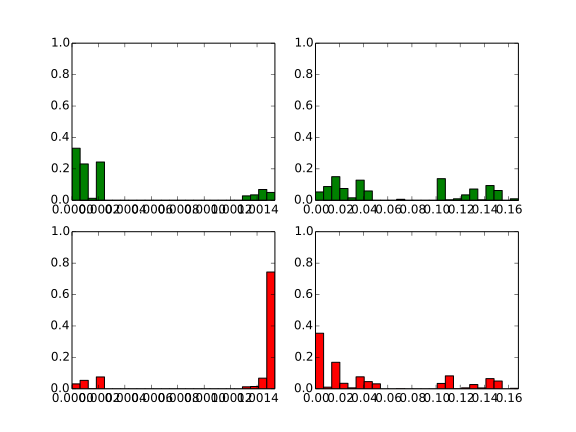
\includegraphics[width =\textwidth]{images/probabilities}
\caption{The distribution in percentages of correct (green) and incorrect (red) document links. Left hand side shows the tag probabilities and the right hand side the link probabilities.}
\label{distribution}
\end{figure}


\subsection{Threshold performance}
\begin{table}
\begin{tabular}{| l | l | l | l | l | l | l | l |}
\hline
THRESHOLD RECALL & Inf. &  Question &  Good Pr.& Project & Person &  Event & {\bf Average} \\
\hline
Textvectorizer & 12.05 & 39.65 & 19.64 & 20.73 & 5.21 & 21.43 & {\bf 15.66}\\
Weighted text & 14.80 & 29.82 & 19.64 & 24.37 & 5.24 & 21.43 & {\bf 15.11}\\
Simple tag & 54.97 & 20.61 & 32.14 & 30.73 & 58.21 & 17.86 & {\bf 46.34}\\
Tag smoothing & 55.56 & 20.61 & 42.86 & 34.90 & 63.33 & 33.73 & {\bf 49.56}\\
Glossaries of tags & 36.51 & 23.25 & 21.43 & 36.35 & 50.20 & 44.05 & {\bf 38.80}\\
Weighted tag & 36.52 & 23.25 & 21.43 & 36.35 & 50.20 & 44.05 & {\bf 38.80}\\
Hybrid & 54.97 & 39.65 & 32.14 & 30.73 & 58.21 & 17.86 & {\bf 49.72}\\
\hline

\hline
THRESH PRECISION & Inf. &  Question &  Good Pr.& Project & Person &  Event & {\bf Average} \\
\hline
Textvectorizer & 26.47 & 50.00 & 41.67 & 24.79 & 24.79 & 7.26 & {\bf 24.05}\\
Weighted text & 26.76 & 41.67 & 33.33 & 26.25 & 8.55 & 27.78 & {\bf 23.00}\\
Simple Tag & 64.19 & 17.11 & 37.50 & 62.50 & 39.32 & 33.33 & {\bf 45.09}\\
Tag smoothing & 46.12 & 18.60 & 43.75 & 56.25 & 36.32 & 44.44 & {\bf 38.29}\\
Glossaries of tags & 25.00 & 14.47 & 37.50 & 33.18 & 17.26 & 46.67 & {\bf 22.00}\\
Weighted tag & 25.00 & 14.47 & 37.50 & 33.18 & 17.26 & 46.67 & {\bf 22.00}\\
Hybrid & 64.19 & 50.00 & 37.50 & 62.50 & 39.32 & 33.33 & {\bf 50.93}\\
\hline
\end{tabular}

\caption{Percentage correct links per vectorizer per document type after a k-link measurement}
\label{bayes_table1}
\end{table}

The performance of the automated threshold was measured for all vectorizers with the metric that gave the best results without threshold - cosine for the text-based descriptors and correlation for the tag-based descriptors. Now, precision and recall are different because the threshold can return a different number of links than the links that are known to be correct. Table xx shows the precision and recall for each of the vectorizers, including an unraveling for each type of document. A comparison between this table and table xx, which is measured with the k-link metric, shows that for the text-vectorizers performance decreases slightly when the threshold value is used. % Tell something about average number of differences in links & draw conclusions from unraveling
For the tag-based vectorizers, both precision and recall drastically improve. Note that precision and recall, with our way of measuring, the average precision and recall per document. Thus, the precision and recall can in fact improve because for some documents recall improves drastically and for some documents precision improves. This explains why the final performance of 46.3\% precision and 43.5\% recall for the simple text vectorizer can be reached. % Tell something about average number of differences in links & and draw conclusions from unraveling

In figure~\ref{fig:thresholds}, the distances for nearby documents the system recommends can be viewed. On the horizontal axis, the documents are shown in sorted order. The vertical axis displays the cosine distance for that document has from the new document. The patterns for all vectorizers seem very noisy, especially for documents that had very little links in the original document. The documents which had more links in the original dataset seem to be less scattered and more plausible to fit to a line.

\begin{figure}[h!]
\begin{tabular}{cc}
\includegraphics[width =0.5\textwidth]{images/thresh_cosine_glossaries_of_tags} 		& \includegraphics[width =0.5\textwidth]{images/thresh_cosine_textvectorizer} \\ \relax
\includegraphics[width =0.5\textwidth]{images/thresh_cosine_weighted_tagvectorizer}	& \includegraphics[width =0.5\textwidth]{images/thresh_cosine_weighted_text_vectorizer} \\ \relax
\includegraphics[width =0.5\textwidth]{images/thresh_cosine_simple_tag_similarity} 	& \includegraphics[width =0.5\textwidth]{images/thresh_cosine_tag_smoothing}
\end{tabular}
\caption{The sorted distances of nearest neighbors and their distance for differend vectorizers. The blue purple gradient represents documents with 0 links (blue) to $\>10$ links (purple)}
\label{fig:thresholds}
\end{figure}


\begin{figure}[h!]
\begin{tabular}{cc}
\includegraphics[width =0.5\textwidth]{images/thresh_cosine_glossaries_of_tags_distances} 		& \includegraphics[width =0.5\textwidth]{images/thresh_cosine_textvectorizer_distances} \\ \relax
\includegraphics[width =0.5\textwidth]{images/thresh_cosine_weighted_tagvectorizer_distances}	& \includegraphics[width =0.5\textwidth]{images/thresh_cosine_weighted_text_vectorizer_distances} \\ \relax
\includegraphics[width =0.5\textwidth]{images/thresh_cosine_simple_tag_similarity_distances} 	& \includegraphics[width =0.5\textwidth]{images/thresh_cosine_tag_smoothing_distances}
\end{tabular}
\caption{Distance betweeen two nearest neighbors sorted by document rank. The blue purple gradient represents documents with 0 links (blue) to $\>10$ links (purple)}
\label{fig:thresholds_differences}
\end{figure}


% Conclusion
\section{Conclusion}
This report has compared six different ways (vectorizers) of converting a text
document into a vector representation and five ways of computing the distance
between these vectors. All this is done in the context of the Starfish network.
Also a method to take the knowledge from the network into account and a way to
determine the number of documents to retrieve were proposed. These combined
form a complete `pipeline' to compute and propose links to known documents for
a new document that is about to be added to the Starfish network.

\begin{itemize}
\item The textvectorizers are significantly better on questions, but do not
  perform well on persons. Additionally, there are issues with future
  applicability (videos, images ect.)
\item The tagvectorizers perform much better on persons. Of all, the simple tag
  vectorizer surprisingly performs the best and is the fastest, so we recommend
  using that one, except for events where the glossaries of tags is better. 
\item The threshold value performs ??
\item The bayesian layer seems to make a too sharp distribution and has no
  promising results. There seems to be no correlation between the correct links
  and their probabilities. Maybe a bigger data set is needed, maybe there is
  really no correlation. 
\item Main conclusion: use text vectorizer for questions and the tagvectorizers
  for others. The bayesian approach does not seem to have the preferred effect.
  The threshold value works acceptable. 
\end{itemize}

% goed product vision recommender system


% MUCH FUTURE WORK!
\section{Future Work \& Recommendations}
Latent dirichlet allocation because tags in dataset are not so good.

Also create incoming links




% Marshall Matters
\bibliographystyle{apalike}
\bibliography{references.bib}


\end{document}
